\chapterimage{metricas.jpg} % Table of contents heading image
\chapter{Diagrama de sistemas y métricas}
\section{Diagrama de sistemas}
Los diagramas de sistemas representan un concepto clave en la búsqueda de la organización y la agrupación de elementos, un ordenamiento hecho a partir de características particulares. En el lenguaje común, estos diagramas se denominan diagramas de paquetes, y dado que los paquetes contienen clases, entonces el diagrama refleja la estructura y la naturaleza del sistema en cuestión.

Los paquetes agrupan las clases de acuerdo a un parámetro de afinidad establecido por la elección del carácter del sistema, la estructura de su concepción y la organización personalizada del proyecto. Ahora bien, ese parámetro de afinidad se llama cohesión y determina el grado de correlación entre las clases para el cumplimiento del objetivo del sistema.

\begin{figure}[H]
	\centering
	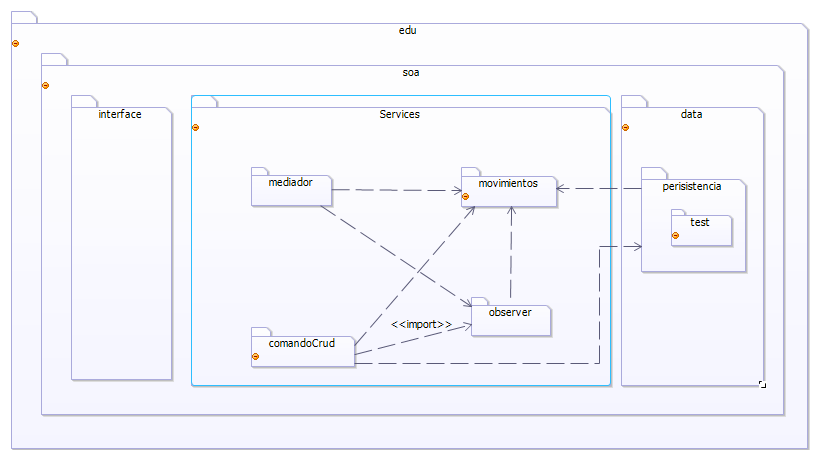
\includegraphics[width=0.9\linewidth]{parte2/imgs/DiagramaSistema/diagramaSistemas}
	\caption{Diagrama del sistema*}
	\label{fig:diagramasistemas}
\end{figure}

\begin{flushright}
	\textit{*Tanto el diagrama como los siguientes parámetros son ofrecidos por el software \textbf{Coloso}.}
\end{flushright}

Dentro de los posibles tipos de carácter que se pueden encontrar para asignarle a un proyecto esta 'com', cuándo la aplicación tiene objetivos lucrativos o comerciales, 'edu' cuando el trabajo se enmarca en cuestiones educativas, 'inv' si se involucra con investigaciones, 'gov' si entidades gubernamentales son el objetivo, entre otras. 

Existen varios tipos de arquitectura para clasificar un proyecto, dentro de los cuales se puede mencionar MVC, PAC, CORBA, SOA, de 2 niveles, de tres, etc.

Finalmente, la organización personalizada involucra de forma directa a las necesidades particulares que el proyecto requiere, por lo que no existen modelos pre-establecidos ni plantillas para usar sino que interviene el criterio personal.

El anterior diagrama de sistemas muestra la jerarquía entre paquetes, todo el proyecto encapsulado en el paquete 'edu', luego en segundo nivel de jerarquía esta la arquitectura, en este caso 'soa' ya que se busca proveer servicios desde la aplicación En la capa de datos se encuentra la persistencia, mostrada como un facade de distintos tipos de persistencia (inicialmente una de test), y requiere de clases del paquete de movimientos para estandarizar la salidas de las consultas y las entradas para actualización y creación Para el CRUD sobre la base de datos se usa el paquete comandoCrud, que trabaja sobre la forma de persistencia seleccionada, y también requiere del modulo observer ya que en cada operación sobre persistencia, y esta notifica al mediador encargado de la gestión entre flujo y sugerencias (que se encuentran el modulo movimientos). Actualmente no cuenta con salidas exteriores de interfaz.\newpage

%%%%%%%%%%%%%%%%%%% seccion 6,2 %%%%%%%%%%%%%%%%%%
\section{Métricas}
Las métricas son paramétros que establecen el nivel de calidad de un sistema, una de ellas es la inestabilidad de los paquetes y se determina a partir del grado de acoplamiento aferente (hacia afuera) y eferente (hacia adentro) de un paquete y la relación entre los mismos. Estas métricas fueron propuestas por Robert Cecil Aka en el año de 1995.

Tomando como base un paquete concreto, el acoplamiento aferente hace referencia a cuando otro paquete hace uso de atributos y/o métodos de clases de dicho paquete o hereda alguna de ellas y el acoplamiento eferente se produce cuando dicha clase hace uso de atributos y/o métodos de clases de otro paquete o hereda de clases de otro paquete.

Estas métricas relacionada con el acoplamiento surgen debido a la relación estrecha entre este, la complejidad, la mantenibilidd y la selección de clases dónde hay que prestar más atención a la hora de realizar pruebas unitarias.

Un elevado acoplamiento aferente se traduce en un paquete con un alto grado de responsabilidad. La responsabilidad y la estabilidad son dos conceptos que están unidos, esto debido a que al existir un elevado número de clases que dependen de clases del paquete, se tiene que ser más prudente a la hora de realizar modificaciones en clases del paquete, debido a los posibles efectos colaterales que se pueden generar.

El alto acoplamiento eferente tiene que ver es con un paquete con un alto grado de dependencia, término asociado con la inestabilidad ya que el funcionamiento de las clases del paquete dependen del comportamiento de clases externas, lo que las hace susceptibles de efectos colaterales en las modificaciones de las mismas y por tanto su funcionamiento encierra una mayor incertidumbre.

La inestabilidad de un paquete se representa a través de la siguiente fórmula:$$I=\frac{C_e}{C_e+C_a}$$ dónde $I$ es inestabilidad, $C_e$ es acoplamiento eferente y $C_a$ es acoplamiento aferente. Por lo tanto la inestabilidad se encontrará en un rango entre 0 y 1.

Estudiando los valores extremos podemos afirmar que si la inestabilidad de un paquete es 1 quiere decir que el acoplamiento aferente es 0 o lo que es lo mismo ninguna clase externa al paquete tiene una relación de dependencia respecto a una clase del paquete, por lo que el paquete sólo tiene dependencias hacia clases externas al paquete. El valor 1 indica una inestabilidad “extrema” del paquete (no obstante, habría que valorar también el valor individual del acoplamiento eferente, ya que, es una opinión personal mía, no todas las inestabilidad con valor 1 tendrían por qué ser iguales) ya que por un lado su comportamiento depende de clases externas, lo cual la hace posible víctima de efectos colaterales y por otro el hecho que no haya clases que dependan del paquete, da una mayor libertad a la hora de realizar modificaciones en el mismo ya que no hay que pensar en terceras clases a la hora de realizar modificaciones en el mismo (también habría que matizar esto, ya que puede haber dependencias entre clases del paquete, medibles mediante distintas métricas, que provoquen que no sea tan ágil o sencillo modificar el paquete)\cite{Pw8M}.

\paragraph{Uso de Eclipse}
Para tener una percepción más visual sobre las métricas de nuestro programa, acudimos al software ECLIPSE, dado que en éste vamos a programar nuestras clases y paquetes, y con ayuda de un plúgin especializado en métricas llamado STAN, hallamos los diagramas de composición, de polución y una grafica de distancia entre inestabilidad y abstracción.

\paragraph{Diagramas de Composición}

La vista de composición permite mirar en el artefacto seleccionado, para ver todos sus contenidos y las dependencias entre ellos. Puede investigar dependencias entre miembros de una clase, clases de un paquete, paquetes, hijos de un árbol de paquetes y entre librerías\cite{Pw9Cmp}.

\begin{figure}[H]
	\centering
	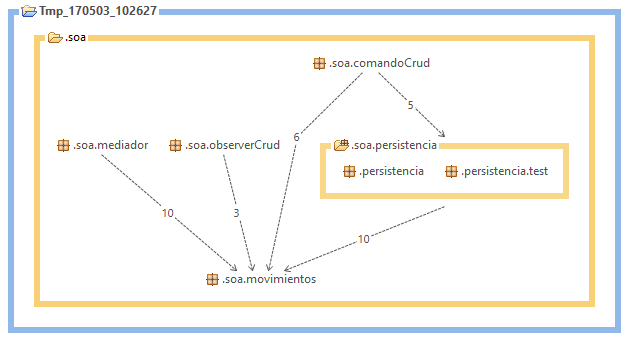
\includegraphics[width=1\linewidth]{parte2/imgs/Metricas/diagramaComposicion}
	\caption{Diagrama de composición del sistema}
	\label{fig:composicion}
\end{figure}

Dado que se puede navegar por cualquiera de los artefactos mostrados, a  continuación mostraremos los diagramas de composición de cada paquete.

\begin{figure}[H]
	\centering
	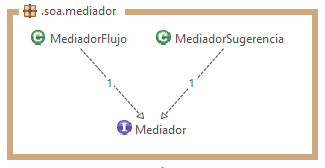
\includegraphics[width=0.7\linewidth]{parte2/imgs/Metricas/SoaMediador}
	\caption{Diagrama de composición del paquete mediador}
	\label{fig:soamediador}
\end{figure}

\begin{figure}[H]
	\centering
	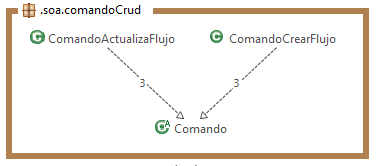
\includegraphics[width=0.7\linewidth]{parte2/imgs/Metricas/SoaComandoCrud}
	\caption{Diagrama de composición del paquete comando}
	\label{fig:soacomandocrud}
\end{figure}

\begin{figure}[H]
	\centering
	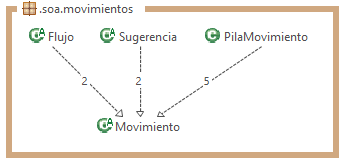
\includegraphics[width=0.7\linewidth]{parte2/imgs/Metricas/SoaMovimientos}
	\caption{Diagrama de composición del paquete Movimientos}
	\label{fig:soamovimientos}
\end{figure}

\begin{figure}[H]
	\centering
	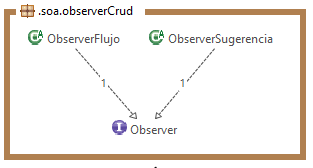
\includegraphics[width=0.5\linewidth]{parte2/imgs/Metricas/SoaObserverCrud}
	\caption{Diagrama de composición del paquete ObseverCrud}
	\label{fig:soaobservercrud}
\end{figure}

\begin{figure}[H]
	\centering
	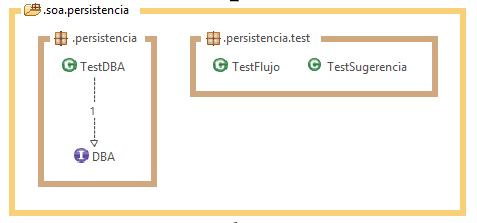
\includegraphics[width=0.7\linewidth]{parte2/imgs/Metricas/SoaPersistencia}
	\caption{Diagrama de composición del paquete de Persistencia}
	\label{fig:soapersistencia}
\end{figure}

\paragraph{Diagrama de Polución}

Un artefacto se dice que viola una métrica si se califica ámbar o rojo para esa métrica. Para cada artefacto, STAN muestra todas las métricas que son violadas por el propio artefacto o por artefactos contenidos.

STAN asume que las violaciones en artefactos "grandes" son peores que las violaciones en "pequeñas": debería ser más relevante si un paquete recibió una mala calificación para alguna métrica A que si una de sus 42 clases recibió una calificación similar para alguna métrica B .Además, incluso si un paquete es calificado ámbar para A, esto podría ser más relevante que si una de sus clases tiene un valor rojo para B\cite{Pw10V&P}.

Para tener esto en cuenta, STAN prioriza una infracción métrica ponderando su clasificación con la cantidad del código subyacente del artefacto. El resultado se muestra en la vista Violaciones.

\begin{figure}[H]
	\centering
	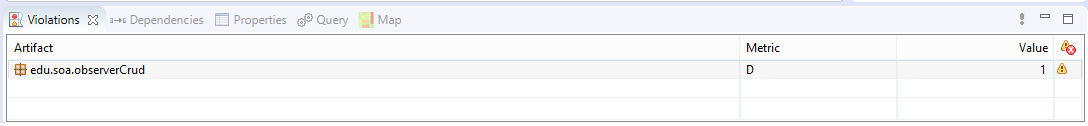
\includegraphics[width=0.8\linewidth]{parte2/imgs/Metricas/violaciones}
	\caption{Violaciones de los artefactos del sistema}
	\label{fig:violaciones}
\end{figure}

Por último, para un determinado artefacto, es posible que desee obtener una idea de cómo las métricas contribuyen a sus violaciones y lo mal que el artefacto está contaminado por las violaciones. Ésto se puede ver el gráfico de contaminación o polución de STAN, en el cual,Cuanto más ancho sea el anillo, mayor será el grado de contaminación del código subyacente. En el nivel de aplicación, el espesor del anillo puede servir como indicador rápido de la calidad estructural global de la base de código\cite{Pw10V&P}.

A continuación podemos ver el diagrama de polución para el sistema: 

\begin{figure}[H]
	\centering
	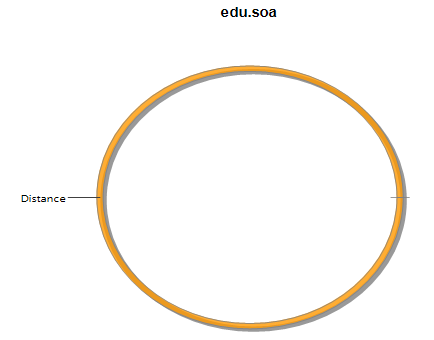
\includegraphics[width=0.6\linewidth]{parte2/imgs/Metricas/diagramaPolucion}
	\caption{Diagrama de polución del sistema}
	\label{fig:polucion}
\end{figure}

\begin{figure}[H]
	\centering
	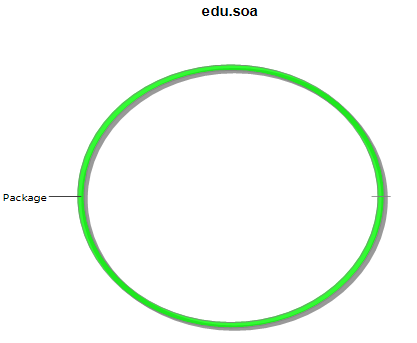
\includegraphics[width=0.6\linewidth]{parte2/imgs/Metricas/diagramaPolucionDominio}
	\caption{Diagrama de polución del sistema según los paquetes}
	\label{fig:polucionDominio}
\end{figure}

Dado que el único artefacto que tiene una violación es el paquete de ObserverCrud, es imprescindible visualizar la polución de éste:

\begin{figure}[H]
	\centering
	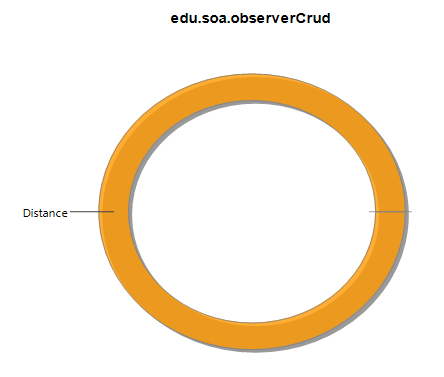
\includegraphics[width=0.6\linewidth]{parte2/imgs/Metricas/diagramaPolucionObserver}
	\caption{Diagrama de polución del paquete ObserverCrud}
	\label{fig:diagramapolucionobserver}
\end{figure}

\begin{figure}[H]
	\centering
	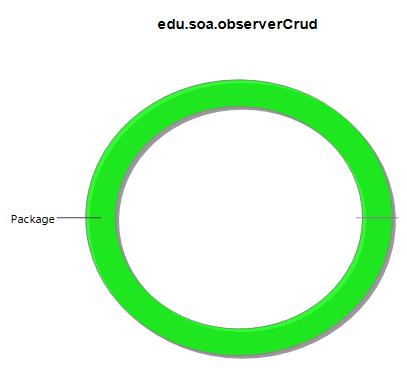
\includegraphics[width=0.6\linewidth]{parte2/imgs/Metricas/diagramaPolucionDominioObserver}
	\caption{Diagrama de polución del paquete ObserverCrud según los paquetes}
	\label{fig:diagramapoluciondominioobserver}
\end{figure}

\paragraph{Grafica de distancia}

Robert C. Martin propuso la idea de que para un software bien diseñado debe haber una relación específica entre dos medidas de paquete: la abstracción de un paquete, que expresará la porción de tipos abstractos contenidos, y su estabilidad, que indica si el paquete es principalmente Utilizado por otros artefactos (estable) o si depende principalmente de otros artefactos (inestables)\cite{Pw11D}.

La relación deseada se captura en el principio de abstracción estable : Un paquete debe ser tan abstracto como estable.

Siguiendo este principio, evitamos obtener paquetes que son utilizados en gran medida por el resto de la aplicación y que, al mismo tiempo, tienen un bajo grado de abstracción. Estos paquetes son una fuente constante de problemas, ya que son difíciles de cambiar o extender.

\begin{itemize}
	\item \textbf{La Abstracción} A para el paquete P se calcula como la relación entre el número de tipos abstractos contenidos en P y el número total de tipos en P. Así, los valores resultantes van desde cero (sólo clases concretas) a uno (sólo interfaces y clases abstractas).
	\item \textbf{La Inestabilidad} I para el paquete P se calcula como la relación entre el número de clases fuera de P requerido por P y el número total de clases fuera de P relacionadas con P. Como anteriormente, los valores resultantes van desde cero (sólo dependencias entrantes) a uno (sólo dependencias salientes).
\end{itemize}

Así que ahora tenemos todo junto para definir la Distancia D , que indica cuán lejos está un paquete de la Secuencia Principal:

$$D=A+I-1$$

Calculando la distancia de esta manera, obtenemos valores entre -1 y 1. Un valor cero significa que el paquete se encuentra exactamente en la Diagonal Principal, el signo indica si el paquete se encuentra por encima o por debajo de la Secuencia Principal. Una métrica derivada, la Distancia Absoluta (| D |), omite el signo, permitiendo así calcular valores medios significativos para artefactos de mayor nivel.

La tabla de distancias STAN le muestra dónde están sus paquetes en vivo, si están ubicados cerca de la Secuencia Principal, como se desee, o si tienden a deslizarse hacia las malas esquinas. Cada paquete se muestra mediante una burbuja, cuyo tamaño está determinado por el número de clases del paquete. El color de la burbuja refleja la clasificación del valor de distancia del paquete, que es, como siempre, ajustable a sus necesidades\cite{Pw11D}.

La siguiente es la distancia de nuestros paquetes en la gráfica de STAN:S

\begin{figure}[H]
	\centering
	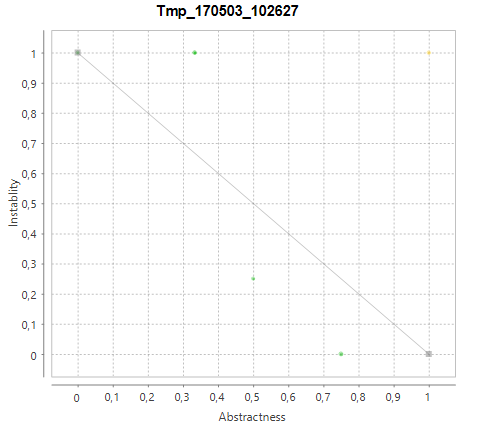
\includegraphics[width=0.7\linewidth]{parte2/imgs/Metricas/diagramaDistancia}
	\caption{Diagrama de distancia del sistema}
	\label{fig:distancia}
\end{figure}